% !TEX program = xelatex
% =====================================================================
%  보스 레이드 협동 NPC를 위한 실패 비용 기반
%  규칙–강화학습 제어권 분리: 경계 재배치와 개입 표본 처리의 실증
%  컴파일: XeLaTeX
%  인용/참고문헌: APA 7th 형식 (수동 서식, biber 불필요)
% =====================================================================
\documentclass[12pt]{article}      % APA 7: 12pt

\usepackage{kotex}                 % 한글 (XeLaTeX 권장)
\usepackage{fontspec}
% --- APA 7 권장 글꼴: 라틴 Times New Roman + 한글 바탕(serif) ---
\setmainfont{Times New Roman}
\setmainhangulfont{Batang}[AutoFakeBold=2.2, AutoFakeSlant=0.2]

\usepackage{geometry}
\geometry{letterpaper, margin=1in}  % APA 7: 1인치(2.54cm) 여백
\usepackage{setspace}
\doublespacing                       % APA 7: 전체 더블 스페이싱
\usepackage{indentfirst}
\setlength{\parindent}{0.5in}        % APA 7: 첫 줄 0.5인치 들여쓰기
\usepackage{enumitem}
\usepackage{tabularx}
\usepackage{booktabs}
\usepackage{ragged2e}
\usepackage{titlesec}
\usepackage{amsmath}
\usepackage{graphicx}
\graphicspath{{figs/}}

% --- 쪽번호 우상단 (APA 7) ---
\usepackage{fancyhdr}
\pagestyle{fancy}
\fancyhf{}
\fancyhead[R]{\thepage}
\renewcommand{\headrulewidth}{0pt}

% --- 표·그림 캡션 APA 7 형식 ---
\usepackage{caption}
\captionsetup[table]{labelfont=bf, textfont=it, labelsep=newline,
  justification=raggedright, singlelinecheck=false, skip=2pt}
\captionsetup[figure]{labelfont=bf, textfont=it, labelsep=newline,
  justification=raggedright, singlelinecheck=false, skip=4pt}

\usepackage[hidelinks]{hyperref}

% --- APA 7 제목 위계 ---
\titleformat{\section}{\normalfont\bfseries\filcenter}{\thesection.}{0.5em}{}
\titleformat{\subsection}{\normalfont\bfseries}{\thesubsection}{0.5em}{}
\titleformat{\subsubsection}{\normalfont\bfseries\itshape}{\thesubsubsection}{0.5em}{}
\titlespacing*{\section}{0pt}{1.2em}{0.4em}
\titlespacing*{\subsection}{0pt}{1.0em}{0.3em}
\titlespacing*{\subsubsection}{0pt}{0.8em}{0.3em}

% --- APA 7 참고문헌: 내어쓰기 0.5인치 ---
\newenvironment{apareferences}
  {\begin{list}{}{%
      \setlength{\leftmargin}{0.5in}%
      \setlength{\itemindent}{-0.5in}%
      \setlength{\listparindent}{-0.5in}%
      \setlength{\itemsep}{0pt}%
      \setlength{\parsep}{0pt}}%
   \raggedright}
  {\end{list}}
\newcommand{\refitem}{\item}

\begin{document}

% =====================================================================
%  APA 7 제목 페이지
% =====================================================================
\thispagestyle{fancy}
\begin{center}
\vspace*{3\baselineskip}
{\bfseries 보스 레이드 협동 NPC를 위한 실패 비용 기반\\
규칙--강화학습 제어권 분리: 경계 재배치와 개입 표본 처리의 실증}

\vspace{2\baselineskip}

박준형\\
메타버스 테크놀로지, 서강대학교 가상융합전문대학원\\
\end{center}

\vspace{2\baselineskip}

\noindent{\bfseries 초록}

\noindent 보스 레이드의 파티원 NPC는 일반 전투 판단뿐 아니라 실패 시 파티 전멸로
이어지는 필수 기믹을 수행해야 한다. 본 연구는 두 가지를 제안한다. 첫째, 보스
레이드 NPC 행동을 \emph{실패 비용}과 \emph{판단의 결정성}이라는 두 축으로
분류하여 행동 트리(behavior tree, BT)와 강화학습(PPO)에 제어권을 배분하는 설계
프레임워크이다. 둘째, 다수 에이전트의 동시 성공을 요구하는 필수 협동 기믹을
결정론적으로 강제하는 보장 계층으로, 위험 행동을 금지하는 기존
실드(shielding)와 개입의 형태가 구별된다. 규칙 개입 턴의 학습 표본 처리는 새로
제안하지 않고, 개입 스텝을 정책 손실에서 제외하는 IARL의 마스킹(F.~Wang et al.,
2018)과 개입 구간 보상을 직전 정책 결정에 할인 누적하는 준마르코프(SMDP)
귀속(Sutton et al., 1999)을 채택한 뒤, 대안 처리(단순 혼합, Drop-only)와 통제
비교하여 채택 근거를 실증하였다. 자체 제작 보스 레이드 게임(Unity + Python
서버, 실제 플레이어 1인과 NPC 3인)의 개정 환경(v2)에서 행동 복제 2{,}000
에피소드와 PPO 20{,}000 에피소드로 학습하고 각 조건을 120 에피소드로 평가한
결과, BT 행동을 정책 표본에 혼합한 조건은 세 역할 모두 정책 엔트로피가 0으로
붕괴하며 승률 0.0\%로 파국적으로 실패한 반면, 개입 표본을 제외한 두
조건(Drop-only 58.3\%, SMDP 귀속 57.5\%)은 동등하게 학습에 성공하였다. 다섯
가지 경계 재배치 실험에서는, 전멸기를 학습으로 이관하면 기믹 보상을 복원해도
학습이 정체되어 승률 0\%에 그친 반면, 낙인 산개는 기믹 성공률을 잃고도 승률이
유지되어 두 분류 축 중 실패 비용이 지배 요인임이 드러났고, 규칙에서 학습으로의
이관은 위험하지만 학습에서 규칙으로의 승격은 관대하다는 경계의 비대칭성이
관찰되었다. 규칙 기반 기준 정책은 동일 v2 환경에서 승률 80.0\%로 하이브리드
구조(57.5\%)보다 높았으며, 격차는 미숙형 플레이어 성향에 집중되었다. 이는 환경
개정 직후 동일 예산 학습의 한계로, 본 연구의 주장은 원시 승률 우위가 아니라
프레임워크의 실증적 검증과 개입 표본 처리의 통제 비교에 있다. 실제 플레이어
대상 사용성 평가는 향후 과제로 남긴다.

\vspace{1\baselineskip}
\noindent \emph{주요어}: 협동 NPC, 보스 레이드, 행동 트리, 강화학습, 제어권 분리,
보장 계층, 개입 표본 처리, PPO
\clearpage

% =====================================================================
\section{서론}
% =====================================================================

MMORPG의 보스 레이드는 탱커, 딜러, 힐러와 같이 역할이 구분된 파티원이 보스의 공격
패턴에 실시간으로 대응하며 협동해야 하는 콘텐츠이다. 파티원의 일부 또는 전부를
NPC로 대체하려는 수요는 꾸준히 존재하지만 --- 예컨대 파티 매칭이 어려운 시간대의
솔로 플레이 지원이나 싱글 플레이어 게임에서의 동료 시스템 --- 상용 게임의 동료
NPC는 대부분 유한 상태 기계(finite state machine, FSM)나 행동 트리(behavior tree,
BT)와 같은 규칙 기반 기법으로 구현된다(Isla, 2005). 규칙 기반 NPC는 동작이 예측
가능하고 필수 행동을 강제할 수 있다는 장점이 있으나, 설계자가 명시하지 않은 상황
--- 파티원 조합의 변화, 플레이어의 실수, 패턴의 중첩 --- 에서 경직된 행동을 보이며,
행동 규칙이 복잡해질수록 유지 보수 비용이 급격히 증가한다.

강화학습(reinforcement learning, RL)은 이러한 경직성을 극복할 대안으로 주목받아
왔다. 대규모 학습을 통해 StarCraft II(Vinyals et al., 2019)와 Dota 2(Berner et
al., 2019)에서 인간 최상위권 수준의 협동 플레이가 달성되었고, 팀 기반 일인칭
게임에서 인간과 함께 플레이할 수 있는 수준의 에이전트도 보고되었다(Jaderberg et
al., 2019). 그러나 보스 레이드 환경에 순수 강화학습을 적용할 때는 이들 연구와
구별되는 구조적 난점이 있다. 보스 레이드의 협동 기믹 --- 예컨대 특정 시점에 전원이
엄폐물 뒤로 숨어야 하는 전멸기 --- 는 (a) 발생 빈도가 낮아 학습 신호가 희소하고,
(b) 파티원 전원의 동시 성공을 요구하며, (c) 단 한 번의 실패가 즉시 에피소드 종료
(전멸)로 이어진다. 탐험 과정의 확률적 정책이 이러한 조건을 우연히 만족하기는
어렵고, 실패가 반복되면 기믹 구간 이전의 전투 행동까지 부정확한 귀인으로 오염된다.

이 난점은 이론적 우려에 그치지 않는다. 저자는 본 연구에 앞서 동일 계열의 보스 전투
환경에서 순수 PPO(Schulman et al., 2017) 기반 역할별 정책을 약 30만 에피소드
학습시키는 사전 실험을 수행하였는데, 전투 승률은 일정 수준에서 정체되었고 특히
협동 기믹의 수행은 학습 후반까지 안정화되지 않았다. 나아가 약 16만 에피소드 이후
정책 엔트로피가 붕괴하면서 성능이 오히려 퇴행하는 현상도 관찰되었다. 보상 설계를
바꾸어 가며 반복한 실험들에서 공통적으로 확인된 것은, 기믹 수행과 전투 판단이라는
성격이 다른 두 과제를 단일 정책의 단일 보상 신호로 동시에 학습시키는 접근 자체의
비효율이었다.

본 연구는 이 관찰로부터, 문제의 근원을 특정 구현 기법의 한계가 아니라 성격이
다른 행동들을 단일 의사결정 방식으로 처리한 데에서 찾는다. 보스 레이드의 NPC
행동은 두 기준으로 분류할 수 있다. 하나는 \emph{실패 비용}, 즉 행동의 실패가
전투 결과에 미치는 영향이고, 다른 하나는 \emph{판단의 결정성}, 즉 주어진 상황에서
올바른 행동이 명확하게 정의될 수 있는 정도이다. 전멸기 발생 시 안전 지점으로
이동하는 행동은 실패 비용이 극단적이고 정답이 명확한 반면, 현재 공격을 지속할지
후퇴할지의 판단은 실패 비용이 상대적으로 낮고 맥락에 따라 최적 행동이 달라진다.
이에 따라 본 연구는 다음의 설계 원칙을 제안한다: \emph{실패 비용이 높고 정답이
명확한 행동은 규칙으로 보장하고, 실패 비용이 상대적으로 낮으며 맥락에 따라 최적
행동이 달라지는 판단은 강화학습으로 적응시킨다}. 이 원칙 하에 제1계층의 결정론적
BT는 전멸기 대응, 임박한 광역기 회피, 낙인 산개와 같은 저빈도·고실패비용
기믹만을 우선순위 규칙으로 확정 처리하는 \emph{보장 계층}으로 동작하고, 규칙에
해당하지 않는 턴은 역할별로 독립된 제2계층 PPO 정책이 담당한다. 기믹이
제1계층에서 보장되므로 제2계층의 보상에서 기믹 항을 제거할 수 있고, 행동 트리는
전체 NPC 행동을 통제하지 않으며, 강화학습은 모든 행동을 처음부터 탐색할 필요
없이 일반 전투 판단에 집중한다.

행동 트리와 강화학습의 결합 자체는 새로운 시도가 아니며, 규칙 기반 제어가
on-policy 학습 알고리즘의 제어권을 일시적으로 대체할 때 발생하는 학습 표본
불일치의 처리 역시 기존 기법이 존재한다. 본 연구는 개입 스텝을 정책 손실에서
제외하는 IARL의 마스킹(F.~Wang et al., 2018)과, 개입 구간의 할인 보상을 직전
정책 결정에 누적하여 가변 길이 준마르코프(semi-Markov) 전이를 구성하는 SMDP
귀속(Sutton, Precup, \& Singh, 1999)을 \emph{채택}한다. 본 연구의 방법론적
기여는 이 처리를 새로 제안하는 것이 아니라, 보장 계층이 상시 개입하는 협동 게임
환경에서 대안적 처리 --- BT 행동을 정책 표본에 그대로 포함하는 단순 혼합과, 개입
턴과 구간 보상을 모두 버리는 Drop-only --- 와 통제 비교하여 채택 근거를 실증하는
데 있다.

제안 구조는 Unity 기반 실시간 클라이언트와 Python 시뮬레이션 서버로 구성된 자체
제작 보스 레이드 게임에 구현되었다. 환경은 11종의 보스 패턴(방향성 근접기, 광역기,
추격 돌진, 카운터 유도기, 패링 유도기, 전멸기 등), 상시 무력화 게이지, 보스 체력에
연동되어 축소되는 전장을 포함하며, 실제 플레이어 1인(딜러)과 NPC 3인(탱커,
힐러, 서포터)이 한 파티를 이룬다. 본 논문은 완료된 실험 결과를 보고한다: 개입
표본 처리의 3조건 통제 비교, 분류 프레임워크가 예측하는 경계를 실제로 옮겨 보는
5종의 경계 재배치 실험, 그리고 동일 환경·동일 프로토콜의 규칙 기반 기준과의
비교이다.

본 연구의 기여는 다음과 같이 요약된다. 첫째, 보스 레이드 NPC 행동을 실패 비용과
판단의 결정성에 따라 규칙 기반 제어와 강화학습 제어로 분리하는 설계 프레임워크를
제안하고, 분류가 예측하는 경계를 다섯 방향으로 실제 재배치하는 실험으로
검증하였다. 이 과정에서 두 축 중 실패 비용이 지배 요인이라는 점과, 규칙에서
학습으로의 이관은 위험하지만 학습에서 규칙으로의 승격은 관대하다는 경계의
비대칭성을 발견하였다. 둘째, 다수 에이전트의 동시 성공을 요구하는 필수 협동
기믹을 강제하는 보장 계층을 제안하고 실제 플레이 가능한 게임에 구현하였다. 이는
학습 정책의 위험 행동을 금지하는 기존 실드(Alshiekh et al., 2018)와 개입의
형태가 구별된다. 셋째, 규칙 개입 구간의 표본 처리로 IARL 마스킹과 SMDP 귀속을
채택하고, 단순 혼합·Drop-only와의 통제 비교를 통해 개입 표본의 혼합이 정책
엔트로피 붕괴와 승률 0\%로 이어지는 파국적 실패임을 실증하였다. 넷째, 규칙 기반
기준 대비 원시 승률 열세를 포함한 전체 실측 결과를 가감 없이 공개하여, 동일
문제를 다루는 후속 연구의 기준점을 제공한다.

% =====================================================================
\section{관련 연구}
% =====================================================================

\subsection{게임 NPC의 규칙 기반 제어}

FSM과 BT는 상용 게임 AI의 표준적 기법이다. 특히 BT는 우선순위가 있는 조건--행동
규칙을 트리로 구조화하여 복잡한 행동의 조합과 재사용을 용이하게 하며, Halo 2 이후
다수의 상용 게임에서 채택되었다(Isla, 2005). 규칙 기반 제어의 강점은 결정론적
보장이다. 즉 특정 조건에서 특정 행동이 반드시 수행됨을 설계 시점에 확정할 수
있다. 본 연구는 이 강점을 폐기하지 않고, 실패 비용이 극단적인 기믹 구간에
한정하여 활용한다.

\subsection{다중 에이전트 강화학습과 역할}

다중 에이전트 강화학습(MARL)에서는 중앙 집중 학습--분산 실행 패러다임 하에 가치
분해(Rashid et al., 2018)나 중앙 비평가(Lowe et al., 2017)를 통해 협동 행동을
학습하는 접근이 주류를 이룬다. 역할의 관점에서는, 에이전트를 역할 공간에 분화시켜
탐색을 구조화하는 ROMA(T.~Wang et al., 2020)와 같이 역할을 학습의 산물로
창발시키는 연구가 있다. 반면 본 연구의 대상인 보스 레이드는 탱커·힐러·서포터라는
역할이 게임 규칙(스킬 구성, 능력치)으로 사전에 고정되어 있으므로, 역할을
창발시키는 대신 역할별로 독립된 관측·정책·보상을 부여하는 명시적 역할 분리를
채택한다. 이는 각 역할의 행동 공간에서 불가능한 행동(예: 탱커의 회복)을 제거하고
보상 신호를 역할 목적에 정렬시키는 실용적 이점이 있다.

\subsection{규칙과 학습의 하이브리드}

학습 정책에 규칙적 구조를 결합하려는 시도는 여러 형태로 존재한다. 게임 도메인의
BT--RL 결합 연구는 주로 BT가 여러 학습된 스킬 중 하나를 선택하거나, 트리 내부의
특정 노드를 학습으로 대체하거나, 상위 전략은 규칙이 하위 조작은 학습이 담당하거나,
규칙이 학습 정책의 위험 행동을 차단하는 구조를 사용한다. 안전 강화학습 분야의
실드(shielding)는 안전 조건을 위반하는 행동을 규칙이 차단하는
구조이며(Alshiekh et al., 2018), 옵션 프레임워크(Sutton et al.,
1999)는 시간적으로 확장된 행동 단위를 계층화한다. 본 연구의 보장 계층은 실드와
마찬가지로 학습 정책의 상위에서 개입한다. 형식적으로도, 선제적(preemptive)
실드의 안전 행동 집합이 단일 원소로 축소되는 경우 실드는 해당 행동을 강제하는
것과 동일해지므로, 개별 시점의 개입만 보면 두 구조는 수렴한다. 그러나 실드
연구의 문제 설정이 단일 에이전트의 안전 조건 위반 방지인 반면, 본 연구의 개입은
다수 에이전트가 제한 시간 내에 \emph{동시에} 성공해야 하는 협동 제약의
강제이며, 안전 집합의 계산이 아니라 협동 기믹의 도메인 지식을 우선순위 규칙으로
직접 기술한다는 점에서 문제 설정과 구성 방식이 다르다. 게임 도메인에서는 사람의
시연으로 정책을 초기화하는 행동 복제(behavior cloning)가 AlphaStar의 초기
단계에서 대규모로 활용된 바 있으며(Vinyals et al., 2019), 본 연구도 규칙 기반
정책의 시연을 이용한 행동 복제 초기화를 채택한다.

국내에서도 규칙 기반 제어와 강화학습을 결합하려는 시도가 이어지고 있다. 김동주와
고석주(2025a)는 모바일 자동 진행 RPG에서 FSM과 심층 Q-학습을 결합하여 개별 NPC의
전투 성능을 개선하였고, 후속 연구(김동주 \& 고석주, 2025b)는 클라이언트가 FSM과
BT로 즉각적 전술 행동을, 서버가 PPO와 다중 에이전트 강화학습으로 고차원 전략을
담당하는 분산형 하이브리드 구조를 제안하였다. 다만 이들 연구의 계층 분리 기준은
연산 부하와 응답성이며, 규칙이 학습 정책의 제어권을 대체한 구간의 학습 표본
처리는 다루지 않는다. 본 연구는 분리 기준을 실패 비용과 판단의 결정성으로
설정하고, 규칙 개입 구간의 on-policy 표본 불일치를 명시적으로 처리·비교한다는
점에서 구별된다.

\subsection{개입 기반 강화학습과 표본 처리}

외부 제어기가 학습 정책의 제어권을 일시적으로 대체하는 환경에서의 on-policy 표본
처리는 안전 강화학습에서 연구되어 왔다. F.~Wang et al.\ (2018)의
IARL(Intervention Aided Reinforcement Learning)은 무인기 내비게이션에서 인간
조작자가 개입한 스텝의 행동을 정책 손실에서 마스킹하되 가치 함수는 전 구간에서
backup하는 처리를 제안하였으며, 본 연구가 채택한 개입 표본 처리의 직접적
선행이다. 최근에는 안전 필터가 정책 경사 추정에 미치는 영향이 이론적으로
분석되고 있다. Markgraf et al.\ (2026)은 연속 행동 공간의 행동 사영(action
projection) 안전 필터에 대해 필터를 정책의 일부로 볼 것인지 환경의 일부로 볼
것인지에 따른 정책 경사의 차이를 분석하였고, Daneshmand et al.\ (2026)의
SafeExplorer는 회복(recovery) 개입 스텝을 마스킹한 정책 경사의 불편성을 증명하고
개입으로 분절된 가변 길이 세그먼트에 할인 누적을 적용하는, 본 연구의 처리와 같은
계열의 방식을 동시기에 제안하였다. 이들 연구는 모두 단일 에이전트의 안전(위험
상태 회피) 개입을 다루는 반면, 본 연구는 다중 역할 NPC의 협동 기믹을 강제하는
개입을 다루며, 채택한 처리를 대안 처리(단순 혼합, Drop-only)와 게임 환경에서
통제 비교하여 실증한다는 점에서 보완적이다.

\subsection{인간과 함께 플레이하는 에이전트}

학습된 에이전트가 학습 시 경험하지 못한 인간과 협동해야 할 때, 자기 대전(self-play)
상대에 과적합된 정책은 인간 파트너와의 협동에서 성능이 급락할 수 있음이 보고되어
왔다(Carroll et al., 2019). 본 연구의 환경은 파티 4인 중 1인이 실제 플레이어라는
점에서 이 문제에 직접 노출된다. 이에 대응하여 학습 중 플레이어 슬롯을 채우는
스크립트 모델의 성향과 노이즈를 에피소드마다 랜덤화하는 도메인 랜덤화(Tobin et
al., 2017)를 적용하고, 평가를 성향별로 분리하여 보고한다.

보스 레이드를 대상으로 한 국내 연구로, 전준렬과 홍진혁(2025)은 4인 파티 전체를
다중 에이전트 강화학습(MA-POCA)으로 동시 조종하면서 인간 플레이 데이터를 활용해
인간다운 플레이 패턴을 모방하는 접근을 제안하였다. 해당 연구는 파티 전원이 학습
에이전트이고 인간다움의 재현이 목표인 반면, 본 연구는 파티에 실제 플레이어가
포함된 상태에서 NPC가 그와 협동하는 문제를 다루며 기믹 수행의 결정론적 보장을
목표로 한다는 점에서 문제 설정이 다르다.

\subsection{기존 행동 트리--강화학습 결합 연구와의 차이}

단순히 행동 트리와 PPO를 결합했다는 사실만으로는 선행 연구와의 차별성을 확보하기
어렵다. 본 연구가 기존 BT--RL 결합 연구와 구별되는 지점을
표~\ref{tab:diff}에 정리한다. 핵심 차이는 세 가지이다. (a) 행동의 복잡도나 계층
구조가 아니라 실패 비용과 판단의 결정성을 제어권 분리 기준으로 삼고, 그 경계를
재배치 실험으로 직접 검증한다. (b) 규칙 개입 구간을 개별 노드의 학습 문제가
아니라 on-policy 표본 수집의 문제로 다루어, 기존 기법(개입 마스킹과 SMDP 귀속)을
채택하고 대안 처리와 통제 비교한다. (c) 실제 인간 플레이어와 역할이 고정된
NPC가 협동하는 레이드 환경에서, 성능 향상 자체가 아니라 기믹 보장과 적응적
협동의 양립을 평가 목표로 삼는다.

\begin{table}[t]
\caption{기존 행동 트리--강화학습 결합 연구와 본 연구의 차이}
\label{tab:diff}
\begin{tabularx}{\textwidth}{lXX}
\toprule
구분 & 기존 BT--RL 결합 & 본 연구 \\
\midrule
분리 기준 & 행동 복잡도나 스킬 종류 & 실패 비용과 판단의 결정성 \\
BT의 역할 & RL 스킬 선택 또는 상위 전략 & 필수 기믹 행동의 직접 보장 \\
RL의 역할 & 개별 스킬 또는 하위 제어 & 역할별 일반 전투 판단 \\
연구 환경 & 단일 에이전트 또는 경쟁 전투 & 인간 1인·NPC 3인의 협동 레이드 \\
역할 구조 & 일반적 NPC 행동 & 탱커·힐러·서포터 역할 고정 \\
필수 기믹 & 제한적으로 다룸 & 전멸 및 동시 성공 기믹 중심 \\
규칙 개입 처리 & 개별 노드 학습 중심 & 개입 마스킹·SMDP 귀속 채택, 대안과 통제 비교 \\
경계 검증 & 고정된 배분 & 5방향 경계 재배치 실험 \\
평가 목표 & 성능 향상, 학습 효율 & 기믹 보장과 적응적 협동의 양립 \\
인간 플레이어 & 없는 경우가 많음 & 실제 인간 플레이어와 협동 \\
\bottomrule
\end{tabularx}
\end{table}

% =====================================================================
\section{연구 질문과 가설}
% =====================================================================

본 연구가 답하고자 하는 연구 질문(RQ)과 그에 대응하는 가설(H)은 다음과 같다.
RQ1--RQ4는 \ref{sec:experiments}절의 완료된 실험으로 답하며, RQ5는 부분적
증거만을 얻었고, RQ6은 향후 과제로 남는다.

\begin{itemize}[leftmargin=0.5in]
\item \textbf{RQ1 (기믹 보장).} 행동 트리 기반 보장 계층은 순수 강화학습
정책보다 보스 레이드의 저빈도·고실패비용 기믹을 안정적으로 수행하는가?
\item \textbf{RQ2 (전투 성능).} 필수 기믹을 행동 트리에 분리한 역할별 PPO는 규칙
기반 NPC와 비교하여 비열등한 전투 성능을 달성하는가?
\item \textbf{RQ3 (개입 표본 처리).} 행동 트리 개입 턴의 표본 처리 방식(단순
혼합, Drop-only, SMDP 귀속)은 학습 안정성과 최종 성능에 어떤 영향을 미치는가?
\item \textbf{RQ4 (제어권 경계).} 실패 비용과 판단의 결정성에 따른 제어권
배분은 실제 경계 재배치 실험의 결과와 일치하는가? 제한된 행동 트리 개입만으로
기믹 성공률을 유지하면서 대부분의 일반 전투 행동을 강화학습 정책에 맡길 수
있는가?
\item \textbf{RQ5 (플레이어 강건성).} 플레이어 성향 도메인 랜덤화를 적용한 협동
NPC는 학습에 사용되지 않은 플레이어 행동 특성에서도 성능을 유지하는가?
\item \textbf{RQ6 (사용자 경험).} 하이브리드 NPC는 순수 규칙 기반 NPC와 비교하여
역할 수행도, 협동성, 상황 적응성 및 신뢰도에서 차이를 보이는가?
\end{itemize}

각 연구 질문에 대응하는 가설은 다음과 같다.

\begin{itemize}[leftmargin=0.5in]
\item \textbf{H1.} 행동 트리가 필수 기믹을 담당하는 조건은 해당 기믹을 학습으로
이관한 조건보다 높은 기믹 성공률을 보일 것이다.
\item \textbf{H2.} 하이브리드 NPC의 보스 레이드 승률은 규칙 기반 NPC와 비교해
비열등할 것이다.
\item \textbf{H3.} 개입 표본을 정책 표본에서 제외하는 방식(Drop-only, SMDP
귀속)은 BT 행동을 표본에 포함하는 단순 혼합 방식보다 안정적인 정책 엔트로피와
높은 최종 성능을 보일 것이다.
\item \textbf{H4.} 하이브리드 NPC는 전체 행동 중 제한된 비율에서만 행동 트리가
개입하더라도 높은 기믹 성공률을 유지할 것이다.
\item \textbf{H5.} 플레이어 성향 랜덤화를 적용한 정책은 단일 플레이어 모델로
학습한 정책보다 미학습 플레이어 성향에서 높은 승률을 보일 것이다.
\item \textbf{H6.} 하이브리드 NPC는 규칙 기반 NPC보다 상황 적응성과 행동 다양성
평가가 높으면서도 예측 가능성과 신뢰도는 유사한 수준을 유지할 것이다.
\end{itemize}

결과를 미리 요약하면, H1(전멸기 이관 실험)·H3(단순 혼합의 붕괴)·H4(개입
24.5\%에서 기믹 85.0\%)는 지지되었고, H2는 개정 환경(v2)의 결과로는 성립하지
않아 기각 내지 보류되었으며(\ref{sec:baseline}절), H5는 성향별 성능을 보고하되
단일 모델 학습과의 대조가 없어 미검증으로 남고, H6은 향후 과제이다.

% =====================================================================
\section{시스템 설계}
% =====================================================================

\subsection{전체 구조}

시스템은 전투 판정을 담당하는 Python 시뮬레이션 서버와 렌더링·조작을 담당하는
Unity 6 클라이언트로 구성된다. 서버는 0.3초 간격의 이산 턴으로 전투를 진행하며,
스냅샷(보스·유닛 상태, 텔레그래프 도형, 이벤트)을 UDP로 클라이언트에 전송하고
플레이어의 행동 명령을 TCP로 수신한다. 조작감을 위해 플레이어의 이동은
클라이언트가 권위를 갖고(20Hz 위치 스트림, 서버는 속도 상한과 충돌만 검증),
피격·명중·쿨다운·기믹 판정 등 전투 결과는 서버가 권위를 갖는 분리 구조를
사용한다. NPC의 의사결정은 전적으로 서버 측에서 수행되므로, 학습 시에는 Unity
없이 서버만 헤드리스로 구동하여 실시간 제약 없이 에피소드를 진행할 수 있다.

\subsection{보스와 전장}

보스는 FSM으로 제어되며 모든 실험 조건에서 동일하게 동작한다. 체력 구간
75\%/50\%에서 페이즈가 전환되고, 50\% 도달 시 전멸기가 강제 발동된다. 패턴은
방향성 근접 연타, 지면 광역기, 표식 대상 추격 돌진(기둥에 유도하여 충돌시키면
그로기), 카운터 유도기(정면에서 카운터 스킬로 저지), 패링 유도기(확산 원을 패링
스킬로 파훼), 낙인(대상이 파티에서 이격해야 함), 전멸기 등 11종이다. 전멸기는 3개
웨이브에 걸쳐 진행되며, 웨이브마다 무작위로 지정되는 안전 석상 뒤 지점에 전원이
22턴의 유예 안에 진입해야 하고, 미진입 유닛은 즉사한다. 상시 무력화 게이지가
존재하여 파티의 누적 타격으로 게이지를 소진시키면 보스가 그로기 상태가 되며,
전장은 25$\times$25 크기로 보스 체력에 연동되어 단계적으로 축소된다.

\subsubsection{환경 개정(v2)}

본 연구는 예비 반복 후 환경을 개정하였다. 개정(v2)의 내용은 (a) 전멸기의 웨이브제
개편(기존 단일 은신 판정 $\rightarrow$ 무작위 안전 석상 3웨이브, 웨이브당 22턴
유예, 미진입 즉사), (b) 전장 25\% 확대(25$\times$25), (c) 힐 쿨다운 4턴
$\rightarrow$ 12턴, 가드 쿨다운 4턴 $\rightarrow$ 8턴 상향이다. 개정의 목적은
전멸기를 1회성 판정에서 반복 협동 판정으로 바꾸고, 회복 자원을 희소화하여 힐
대상 선택의 전략적 비중을 높이는 것이다. \emph{본 논문의 모든 수치는 v2 환경
기준이며}, 개정 전(v1) 환경의 측정치는 \ref{sec:v1}절의 예비 결과 한 건으로만
언급한다.

\subsection{파티와 행동 공간}

파티는 실제 플레이어(딜러)와 NPC 3인(탱커, 힐러, 서포터)으로 구성된다. 관측은
자기 상태, 파티원 상대 상태, 보스 상태(패턴, 남은 시전 턴, 무력화 게이지), 위험
도형 요약 등 132차원 벡터이고, 행동은 정지·8방향 이동·평타·역할 스킬·회피
기동·카운터 등 22종의 이산 행동이다. 역할별 스킬 구성은 게임 규칙으로 고정된다
(탱커: 도발·가드, 힐러: 단일/광역 회복, 서포터: 공격·보호 버프).

% =====================================================================
\section{제안 방법: 실패 비용 기반 제어권 분리와 보장 계층}
% =====================================================================

\subsection{행동 분류 기준: 실패 비용과 판단의 결정성}

제안 프레임워크의 출발점은 구현 난이도가 아니라 행동의 성격에 따른 분류이다.
\emph{실패 비용}은 행동의 실패가 전투 결과에 미치는 영향이다. 공격 위치 선정,
스킬 선택, 회복 시점 판단은 실패해도 손실이 국소적이지만, 전멸기 대응, 제한 시간
내 장판 이탈, 낙인 동시 산개는 한 번의 실패가 파티 전멸로 이어질 수 있다.
\emph{판단의 결정성}은 주어진 상황에서 올바른 행동이 명확하게 정의될 수 있는
정도이다. 전멸기 웨이브에서 지정된 안전 석상 뒤로 이동하는 행동은 정답이 유일하게
정의되는 반면, 현재 공격을 지속할지 후퇴할지는 체력, 쿨다운, 파티원의 위치, 보스
상태에 따라 답이 달라진다. 두 기준에 따른 제어 방식의 배분을
표~\ref{tab:criteria}에 정리한다. 필수 기믹은 발생 빈도가 낮아 강화학습의 탐색
대상으로 삼기 어렵고 다수 NPC의 동시 성공을 요구하므로 규칙으로 보장하는 것이
적합한 반면, 일반 전투 판단은 고빈도로 반복 경험이 가능하고 플레이어 성향에 따라
행동이 달라져야 하므로 학습이 적합하다. 이 원칙을 통해 강화학습은 모든 행동을
처음부터 탐색할 필요가 없으며, 행동 트리는 전체 NPC 행동을 통제하지 않고 반드시
성공해야 하는 일부 구간만 담당한다. 이 분류가 실제 경계와 일치하는지는
\ref{sec:boundary}절의 경계 재배치 실험으로 검증한다.

\begin{table}[t]
\caption{행동 특성에 따른 제어 방식 배분}
\label{tab:criteria}
\begin{tabularx}{\textwidth}{Xl}
\toprule
행동 특성 & 적용 방식 \\
\midrule
실패 비용이 높고 정답이 명확함 & 행동 트리 \\
실패 비용이 낮고 상황 의존적임 & 강화학습 \\
저빈도이며 탐색이 어려움 & 행동 트리 \\
고빈도이며 반복 경험이 가능함 & 강화학습 \\
모든 NPC의 동시 성공이 필요함 & 행동 트리 \\
플레이어 성향에 따라 행동이 달라짐 & 강화학습 \\
\bottomrule
\end{tabularx}
\end{table}

\subsection{제1계층: 기믹 보장 계층}

제1계층은 매 턴 우선순위 순서로 평가되는 결정론적 규칙 집합이다. 규칙이 발화하면
해당 행동이 확정되고, 어떤 규칙도 발화하지 않으면 제어가 제2계층으로 넘어간다
(표~\ref{tab:bt}). 규칙은 발생 빈도가 낮고 실패 비용이 큰 기믹에 한정하며,
일반적인 포지셔닝·공격·회복 판단은 의도적으로 포함하지 않는다. 특히 임박 위험
회피 규칙은 위험 도형 안에 있더라도 발동까지 여유가 있으면(잔여 3턴 이상) 발화하지
않는데, 이는 ``위험을 미리 벗어나는 선제적 포지셔닝''을 제2계층의 학습 대상으로
남겨 두기 위함이다. 이 계층은 학습 정책이 선택한 위험 행동을 사후에 차단하는
실드가 아니라, 협동 기믹 국면에서 필수 행동을 선제적으로 강제하는 보장
계층으로 동작한다.

\begin{table}[t]
\caption{제1계층 보장 계층의 우선순위 규칙}
\label{tab:bt}
\begin{tabularx}{\textwidth}{clX}
\toprule
순위 & 규칙 & 조건 $\rightarrow$ 행동 \\
\midrule
1 & 전멸기 대응 & 전멸기 웨이브 진행 중 $\rightarrow$ 현 웨이브의 안전 석상 뒤 지점으로 이동 \\
2 & 임박 위험 회피 & 위험 도형 안 $\wedge$ 발동 잔여 $\le 2$턴 $\rightarrow$ 최단 탈출
    (탱커는 가드 가능 시 가드) \\
3 & 낙인 산개 & 낙인 대상 $\rightarrow$ 파티로부터 이격 이동 \\
4 & 무력화 집중 & 보스 그로기 $\rightarrow$ 근접 확보 후 집중 공격 (탱커는 도발 우선) \\
5 & 패링 장판 탈출 & 패링 유도 원 안 (NPC는 패링 불가) $\rightarrow$ 원 밖 탈출 \\
6 & 돌진 유도 & 추격 돌진 표식이 자신 $\rightarrow$ 기둥 후방으로 이동해 충돌 유도 \\
--- & 위임 & 어느 규칙도 미발화 $\rightarrow$ 제2계층(RL) \\
\bottomrule
\end{tabularx}
\end{table}

\subsection{제2계층: 역할별 PPO}

제2계층은 탱커·힐러·서포터 각각 독립된 액터--크리틱 네트워크(공유 은닉 2층
256유닛)로 구성되며 PPO로 학습된다. 보상은 팀 공통 항(보스 처치, 파티 생존,
시간 페널티)과 역할 항(탱커: 어그로 유지, 힐러: 유효 회복과 위급 대상 우선,
서포터: 버프 적중과 보조 딜)의 합이며, 위험 도형 안에 있는 동안은 양(+)의 역할
보상이 차단되어 회피가 우선되도록 한다. 중요한 설계는 기믹 관련 보상(전멸기 대응,
산개, 카운터, 돌진 유도 등)을 제2계층 보상에서 전부 제거한 것이다. 기믹은
제1계층이 보장하므로, 제2계층은 순수 전투 보상만으로 학습하여 신호가 명료해지고
탐색 공간이 줄어든다.

\subsection{규칙 개입 구간의 표본 처리: 개입 마스킹과 SMDP 귀속의 채택}
\label{sec:sampling}

학습 중에도 제1계층은 활성 상태이므로, 롤아웃에는 RL이 결정한 턴과 BT가 결정한
턴이 섞여 있다. PPO는 현재 정책이 생성한 행동 표본을 전제로 하는 on-policy
알고리즘이므로, BT가 선택한 행동 $a_t$를 상태 $s_t$ 및 정책에서 계산한 로그 확률
$\log \pi(a_t \mid s_t)$와 함께 표본에 그대로 저장하면, 실제 행동 생성 주체는
BT임에도 정책이 생성한 행동처럼 취급되어 정책 경사 추정이 오염될 수 있다.

이를 피하기 위해 BT가 개입한 턴은 정책 학습 표본에서 제외한다. 그러나 해당
구간에서 발생한 보상까지 제거하지는 않는다. 시각 $t$의 RL 결정 이후 BT 개입
등으로 다음 RL 결정까지 $k$턴이 소요되었다면, 그 구간의 보상을 직전 RL 결정에
누적하여 하나의 가변 길이 전이 $(s_t, a_t, R_t^{(k)}, s_{t+k})$를 구성한다. 누적
보상은 할인 합
\begin{equation}
R_t^{(k)} = \sum_{i=0}^{k-1} \gamma^{i}\, r_{t+i}
\label{eq:smdp-return}
\end{equation}
으로 정의되며, 여기서 $r_{t+i}$는 각 턴에서 발생한 보상, $\gamma$는 할인율,
$k$는 다음 RL 결정까지의 턴 수이다. BT가 개입하지 않은 턴에서는 $k=1$이 되어
일반적인 1턴 전이와 일치한다. 가치 추정 역시 1턴 전이가 아니라 가변 길이 전이에
대한 시간차 오차
\begin{equation}
\delta_t^{(k)} = R_t^{(k)} + \gamma^{k} V(s_{t+k}) - V(s_t)
\label{eq:smdp-delta}
\end{equation}
를 사용하며, 이점(advantage) 추정도 동일한 가변 길이 전이 위에서 수행된다.

강조하건대 이 처리는 본 연구의 새로운 제안이 아니라 기존 기법의 채택이다. 개입
스텝의 행동을 정책 손실에서 제외하는 마스킹은 IARL(F.~Wang et al., 2018)에서,
가변 길이 전이에 대한 할인 누적과 $k$-스텝 부트스트랩은 준마르코프 결정 과정과
옵션 프레임워크(Sutton et al., 1999)에서 가져온 것이다. 이 구조에서 하나의 RL
결정은 ``다음 RL 결정까지의 구간''을 갖는 시간 확장 행동으로 해석된다. 본 연구의
기여는 이 조합을 보장 계층이 상시 개입하는 협동 게임 환경에 적용하고, 대안적
처리 --- BT 행동을 표본에 그대로 포함하는 단순 혼합과, 개입 턴과 구간 보상을 모두
버리는 Drop-only --- 와의 통제 비교(\ref{sec:def}절)로 채택 근거를 실증하는 데
있다.

\subsection{학습 절차}

학습은 다음 요소를 결합한다. (a) \emph{행동 복제 초기화}: 규칙 기반 기준 정책
(FSM)의 시연 2{,}000 에피소드로 각 역할 네트워크를 교차 엔트로피 손실로 사전
학습한다. (b) \emph{커리큘럼}: 보스 체력을 12{,}000 $\rightarrow$ 28{,}000
$\rightarrow$ 55{,}000(실전 값)의 3단계로 증가시키며, 최근 승률이 40\%에 도달하면
승급한다(Bengio et al., 2009). (c) \emph{플레이어 도메인 랜덤화}: 플레이어 슬롯을
채우는 스크립트 모델의 성향을 에피소드마다 공격형(회피 지연)·안정형(회피
우선)·미숙형(확률적 오행동)에서 샘플링하고 이동 지터·스킬 지연 노이즈를 부여한다.
(d) \emph{학습--배포 일치}: 배포 시 반응 지연 모사를 위해 관측을 1턴 지연시키므로,
학습 롤아웃에서도 동일한 지연 관측을 사용한다. (e) \emph{엔트로피 감시}: 사전
실험에서 관찰된 엔트로피 붕괴--성능 퇴행을 조기 탐지하기 위해 역할별 정책
엔트로피를 학습 로그에 기록하고, 붕괴 시 이전 체크포인트로 롤백한다.

배포 시(실제 게임) 제2계층에는 행동의 자연스러움을 위한 두 장치가 추가된다. 온도 1.0의
확률적 샘플링(결정론적 argmax 금지)과, 직전 이동 방향에 로짓 보너스를 주는 행동
관성(지터 억제)이다. 학습된 모델이 없는 경우 제2계층은 규칙 기반 정책으로
대체되어 게임은 항상 구동 가능하다.

% =====================================================================
\section{실험}
\label{sec:experiments}
% =====================================================================

\subsection{사전 실험: 순수 강화학습의 실패}

본 연구 설계의 직접적 근거가 된 사전 실험을 요약한다. 동일 계열의 보스 전투
환경에서 역할별 PPO 정책을 기믹 보상을 포함한 단일 보상으로 약 30만 에피소드
학습시켰을 때, (a) 협동 기믹(무력화 시간 창 대응 등)의 수행률이 학습 후반까지
안정화되지 않았고, (b) 약 16만 에피소드 이후 정책 엔트로피가 붕괴하며 승률이
오히려 하락하는 퇴행이 관찰되었다. 이후 관측 설계 변경과 보상 재설계를 결합한
반복 실험(하이브리드 보상 조정 8회)을 통해 승률 56\%, 무력화 기여 37\% 수준까지
개선되었으나, 이는 대규모 반복 튜닝의 결과였으며 기믹의 결정론적 보장은 끝내
확보되지 않았다. 이 경험은 ``기믹 수행을 학습으로 획득하는 것''과 ``기믹 수행을
규칙으로 보장하고 학습은 전투에 집중시키는 것''의 비용 차이를 보여 주며, 본
연구의 2계층 분리 설계로 이어졌다.

\subsection{예비 반복(v1)과 환경 개정}
\label{sec:v1}

개정 전(v1) 환경 --- 단일 은신 판정 전멸기, 힐 쿨다운 4턴 --- 에서 수행한 예비
반복에서 제안 구조는 최종 난이도 승률 70.8\%($n=120$)로 동일 v1 환경의 규칙 기반
기준(64--75\%)과 동등한 수준에 도달하였고, 기믹 성공률 86.9\%, BT 발화 비율
21.8\%를 기록하였다. 이 예비 결과는 구조의 실행 가능성을 확인해 주었으나, v1
환경은 전멸기가 1회성 판정이고 회복 자원이 풍부하여 협동 기믹과 자원 관리의
난이도가 낮았다. 이에 환경을 v2로 개정(전멸기 웨이브제, 전장 25\% 확대, 힐 쿨
4$\rightarrow$12턴·가드 4$\rightarrow$8턴)하고 본 실험을 전부 v2에서 다시
수행하였다. 이하의 모든 수치는 v2 기준이며, v1 수치와 직접 비교할 수 없다.

\subsection{실험 설정과 비교 조건}

모든 조건은 행동 복제 2{,}000 에피소드로 초기화한 뒤 PPO로 학습하였다. 표본
처리 비교 조건(아래 C/D/E)은 20{,}000 에피소드, 경계 재배치 조건(M1--M5)은
10{,}000 에피소드를 학습하였다. 최종 평가는 조건별 120 에피소드로, 보스 체력
55{,}000(실전 값)에서 플레이어 성향(공격형·안정형·미숙형)을 에피소드마다
랜덤화하여 수행하였다. 비교 조건은 다음과 같다.

\begin{itemize}[leftmargin=0.5in]
\item \textbf{조건 A (규칙 기반 NPC).} 모든 기믹과 일반 전투 행동을 FSM으로
구현한 기준 정책. 동일 v2 환경·동일 평가 프로토콜로 평가하였다.
\item \textbf{조건 B (순수 PPO).} 기믹과 일반 전투 행동을 모두 역할별 PPO가
결정한다. v2 환경에서의 재학습은 수행하지 않았으며, 동일 계열 환경의 사전
실험(약 30만 에피소드)으로 갈음한다.
\item \textbf{조건 C (제안 하이브리드).} 필수 기믹은 보장 계층이, 일반 전투는
역할별 PPO가 담당하며, 개입 표본은 아래 조건 F의 방식으로 처리한다. 즉 본
연구에서 조건 C와 F는 동일한 학습 실행이다.
\item \textbf{조건 D (단순 혼합).} 조건 C와 같은 2계층 구조이되, 행동 트리가
개입한 턴도 PPO 학습 표본에 그대로 포함한다.
\item \textbf{조건 E (Drop-only).} 행동 트리가 개입한 턴과 해당 구간의 보상을
모두 제거한다.
\item \textbf{조건 F (SMDP 귀속).} 행동 트리 개입 턴은 표본에서 제외하되 해당
구간의 보상은 직전 PPO 결정에 할인 누적한다(\ref{sec:sampling}절의 채택 방식).
\end{itemize}

\subsection{결과 1: 개입 표본 처리의 통제 비교 (D/E/F)}
\label{sec:def}

표~\ref{tab:def}는 세 가지 표본 처리 조건의 최종 평가 결과를, 그림
\ref{fig:def}은 학습 곡선을 보여 준다. 결과는 명확한 비대칭을 드러낸다.

\begin{table}[t]
\caption{개입 표본 처리 방식의 통제 비교 (v2 환경, $n=120$)}
\label{tab:def}
\begin{tabularx}{\textwidth}{Xrrr}
\toprule
지표 & D. 단순 혼합 & E. Drop-only & F. SMDP 귀속 \\
\midrule
승률 & 0.0\% & 58.3\% & 57.5\% \\
기믹 성공률 & 75.7\% & 86.8\% & 85.0\% \\
BT 발화 비율 & 9.7\% & 24.4\% & 24.5\% \\
평균 처치 턴 & --- & 828.0 & 847.6 \\
정책 엔트로피(탱커/힐러/서포터) & 0.0 / 0.0 / 0.0 & --- & 0.79 / 2.49 / 0.51 \\
탱커 어그로 1위 점유율 & 0.27 & --- & 0.62 \\
\bottomrule
\end{tabularx}
\vspace{2pt}
{\footnotesize \emph{주.} 정책 엔트로피는 학습 종료 시점 값. ---는 해당 없음(D는
전승 실패로 처치 턴이 정의되지 않음) 또는 별도 집계하지 않은 항목.}
\end{table}

\begin{figure}[t]
\centering
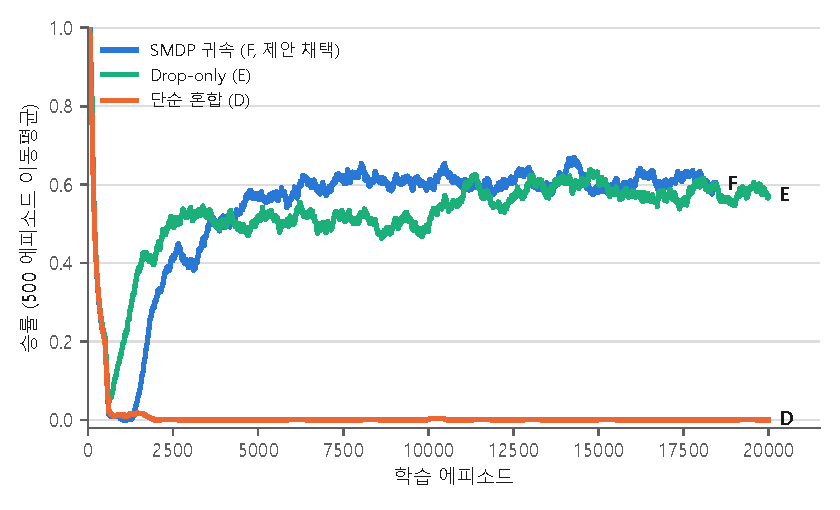
\includegraphics[width=\textwidth]{fig_def_curves.pdf}
\caption{개입 표본 처리 조건별 승률 수렴 곡선(500 에피소드 이동평균). 단순
혼합(D)은 학습 전 구간에서 승률이 형성되지 못한 반면, 개입 표본을 제외한 두
조건(E, F)은 유사한 궤적으로 수렴하였다.}
\label{fig:def}
\end{figure}

첫째, BT 개입 행동을 정책 표본으로 취급한 단순 혼합(D)은 파국적으로 실패하였다.
최종 승률은 0.0\%였고, 세 역할 모두 정책 엔트로피가 0.0으로 붕괴하였으며, 힐러는
판당 힐 시전 0회, 탱커의 어그로 1위 점유율은 0.27(F 조건 0.62)에 그쳤다.
결정론적 BT 행동이 ``정책이 생성한 고확률 행동''처럼 학습되면서 정책 분포 전체가
결정론으로 붕괴한 것으로, 사전 실험에서 관찰된 엔트로피 붕괴--성능 퇴행과 같은
계열의 현상이 표본 오염에 의해 재현된 것으로 해석된다. D 조건의 BT 발화 비율이
9.7\%로 낮은 것은 붕괴된 정책 하에서 에피소드가 조기에 종결되어 기믹 국면 노출
자체가 줄어든 결과로 보인다.

둘째, 개입 표본을 정책 표본에서 제외한 두 조건은 모두 학습에 성공하였고, 최종
성능은 통계적으로 구분되지 않았다(E 58.3\% vs.\ F 57.5\%, $n=120$). 학습
곡선상으로는 F가 다소 앞선 구간이 있었으나(그림~\ref{fig:def}), 120 에피소드
평가에서 그 차이는 표집 오차와 구분할 수 없다. 따라서 본 실험이 지지하는 결론은
다음과 같이 한정된다: \emph{개입 표본을 정책 표본에 혼합하는 것은 치명적이며
제외는 필수이다. 다만 제외 이후 개입 구간 보상의 귀속 방식(버림 vs.\ SMDP
누적)의 차이는 본 환경에서 크지 않았다}. 개입 구간이 짧고 팀 공통 보상이
지연·희소한 본 환경의 특성상 구간 보상의 정보량이 제한적이었을 가능성이 있으며,
개입 구간이 길거나 구간 내 보상 밀도가 높은 환경에서의 재검은 향후 과제이다.

\subsection{결과 2: 경계 재배치 실험 (M1--M5)}
\label{sec:boundary}

분류 프레임워크(표~\ref{tab:criteria})가 예측하는 제어권 경계가 실제와
일치하는지 검증하기 위해, 기준 구성(조건 C)에서 행동 하나씩을 경계 반대편으로
이관한 다섯 조건을 학습하였다. M1--M4는 보장 계층의 규칙을 하나 제거하고 해당
기믹 보상을 RL 보상에 복원하는 규칙$\rightarrow$학습 이관이고, M5는 반대로 RL
소관이던 어그로 관리를 규칙으로 승격하는 학습$\rightarrow$규칙 이관이다.
표~\ref{tab:moved}에 결과를, 그림~\ref{fig:boundary}에 실패 비용$\times$판단
결정성 평면 위의 경계 지도를 정리한다.

\begin{table}[t]
\caption{경계 재배치 실험 결과 (v2 환경, 학습 10{,}000 에피소드, $n=120$)}
\label{tab:moved}
\begin{tabularx}{\textwidth}{lXrrr}
\toprule
조건 & 이관 내용 & 승률 & 대상 기믹 성공률 & 전체 기믹 \\
\midrule
기준(C) & --- & 57.5\% & --- & 85.0\% \\
M1 & 전멸기 $\rightarrow$ RL & 0.0\% & 42\% (기준 87\%) & 84.0\% \\
M2 & 낙인 산개 $\rightarrow$ RL & 57.5\% & 26\% (기준 78\%) & 76.0\% \\
M3 & 임박 회피 $\rightarrow$ RL & 55.0\% & --- & 69.1\% \\
M4 & 무력화 집중 $\rightarrow$ RL & 59.2\% & --- & 87.0\% \\
M5 & 어그로 관리 $\rightarrow$ BT (역방향) & 61.7\% & --- & 86.4\% \\
\bottomrule
\end{tabularx}
\vspace{2pt}
{\footnotesize \emph{주.} 기준(C)은 20{,}000 에피소드 학습이므로 절대 수치
비교에는 주의가 필요하다. 대상 기믹 성공률은 이관된 기믹 자체의 성공률이며,
M3--M5는 별도의 단일 성공률 지표를 정의하지 않았다(M3은 본문의 피격 횟수로
보고).}
\end{table}

\begin{figure}[t]
\centering
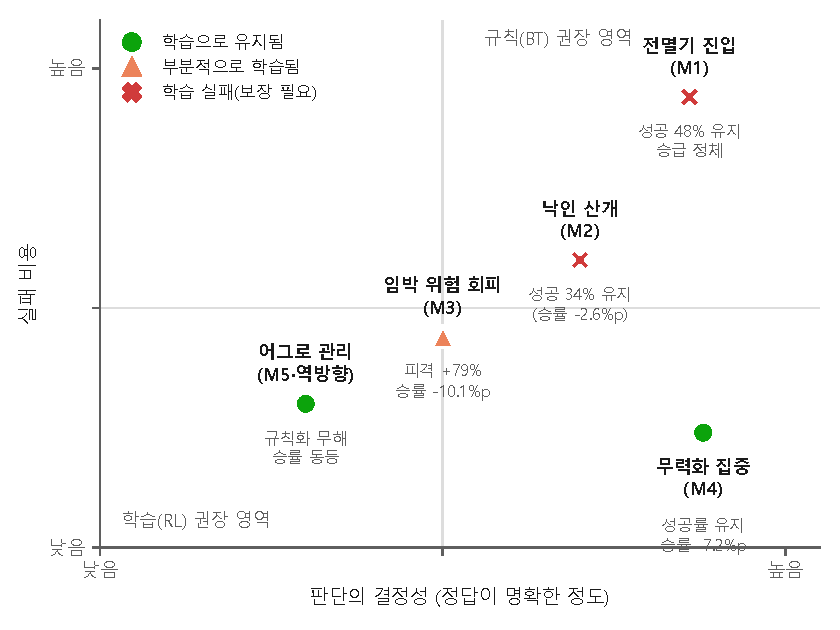
\includegraphics[width=\textwidth]{fig_boundary_map.pdf}
\caption{실패 비용$\times$판단 결정성 평면 위의 제어권 경계 지도. 각 행동의
분류상 위치와 경계 재배치 실험(M1--M5)의 결과를 함께 표시하였다. 실패 비용이
극단적인 영역(M1)의 학습 이관은 파국적으로 실패한 반면, 경계 부근(M4)과 역방향
승격(M5)은 무해하였다.}
\label{fig:boundary}
\end{figure}

\begin{figure}[t]
\centering
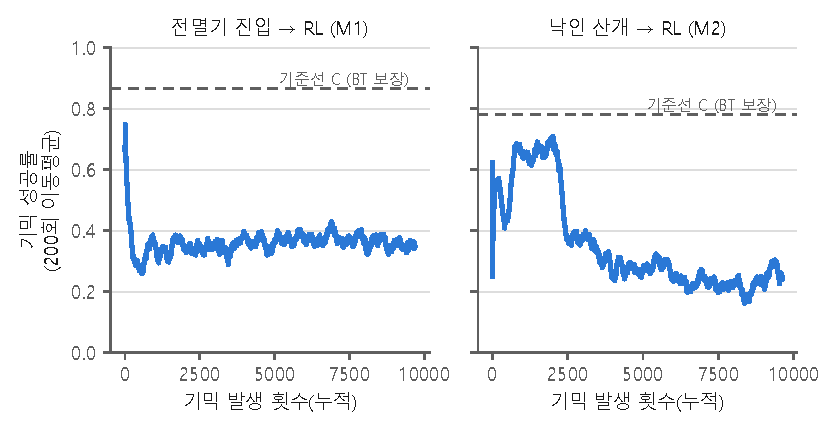
\includegraphics[width=\textwidth]{fig_moved_gimmicks.pdf}
\caption{학습으로 이관된 기믹의 성공률 곡선(M1: 전멸기, M2: 낙인 산개). M2는
행동 복제 웜스타트로 약 70\%의 산개 성공률을 갖고 학습을 시작했으나, PPO 학습이
진행되며 이를 다시 상실하는 망각 궤적을 보였다.}
\label{fig:moved}
\end{figure}

\textbf{M1 (전멸기 $\rightarrow$ RL): 파국적 실패.} 전멸기 규칙을 제거하고 기믹
보상을 복원했음에도 전멸기 성공률은 42\%(기준 87\%)에 그쳤고, 커리큘럼의 보스
체력 28{,}000 단계에서 10{,}000 에피소드 내내 정체하여 최종 난이도 승급에
실패하였으며, 최종 난이도 평가 승률은 0\%였다. 실패 비용이 극단적(미진입 즉사)
이고 저빈도이며 파티 전원의 동시 성공을 요구하는 행동은, 보상을 제공하더라도
탐색으로 확보되지 않았다. 이는 RQ1/H1을 강하게 지지한다.

\textbf{M2 (낙인 산개 $\rightarrow$ RL): 기믹은 잃었으나 승률은 유지.} 낙인 산개
성공률은 26\%(기준 78\%)로 학습에 실패했지만, 승률은 57.5\%로 기준선과 동등했다.
흥미로운 것은 학습 궤적이다(그림~\ref{fig:moved}). 행동 복제 웜스타트 직후 산개
성공률은 약 70\%였으나, PPO 학습이 진행되며 이 행동을 다시 상실하였다. 낙인
실패의 실제 귀결이 광역 피해이지 즉사가 아니어서, 산개 이동의 기회비용(딜 손실,
힐 사거리 이탈)이 실패 페널티를 상회하는 방향으로 정책이 이동한 것으로 해석된다.
즉 이 기믹의 \emph{실제} 실패 비용은 설계 시 가정한 것보다 낮았고, 정답이
명확한(판단 결정성이 높은) 행동임에도 학습이 유지하지 못했다는 점에서, 두 분류
축 중 학습 가능성을 지배하는 요인은 판단의 결정성이 아니라 실패 비용임을
시사한다.

\textbf{M3 (임박 회피 $\rightarrow$ RL): 부분 학습.} 판당 피격 횟수가 72회에서
129회로 79\% 증가했으나, 승률 55.0\%(기믹 69.1\%)로 전투는 유지되었다. 회피는
고빈도 행동이라 학습 신호는 충분했으나 규칙 수준의 신뢰성에는 도달하지 못했다.

\textbf{M4 (무력화 집중 $\rightarrow$ RL): 학습으로 유지.} 전체 기믹 성공률
87.0\%, 승률 59.2\%로 기준선 수준을 유지하였다. 무력화 집중은 그로기 시간 창
동안의 고빈도 공격 행동으로, 분류 평면에서 경계선에 위치한 행동인데, 실제로 RL
소관으로 옮겨도 무해했다.

\textbf{M5 (어그로 관리 $\rightarrow$ BT, 역방향): 무해.} 어그로 관리를 규칙으로
승격한 조건은 승률 61.7\%(기믹 86.4\%, BT 발화 27.6\%)로 기준선과 동등 이상이었다.
판단 결정성이 충분히 높은 행동은 규칙화해도 성능 손실이 없었다.

종합하면 경계에는 \emph{비대칭성}이 있다. 규칙에서 학습으로의 이관은 대상 행동의
실패 비용에 따라 파국적 실패(M1)부터 무해(M4)까지 결과가 갈리는 위험한 방향인
반면, 학습에서 규칙으로의 승격(M5)은 관대하다. 설계 관점에서 이는 ``의심스러우면
규칙에 두라''는 보수적 지침으로 요약되며, 분류 프레임워크의 두 축 중 실패 비용이
일차 기준, 판단 결정성이 이차 기준임을 뜻한다.

\subsection{결과 3: 규칙 기반 기준과의 비교}
\label{sec:baseline}

동일 v2 환경·동일 프로토콜에서 규칙 기반 기준(조건 A)은 승률 80.0\%, 기믹 성공률
76.1\%, 평균 처치 827.2턴(하이브리드 847.6턴), 성향별 승률 공격형 87.0\%·안정형
83.7\%·미숙형 64.5\%를 기록하였다. 제안 하이브리드(조건 C/F)의 승률 57.5\%는
이에 못 미치며, 본 연구는 이 열세를 숨기지 않고 보고한다. 세부를 보면 세 가지
사실이 드러난다. 첫째, 격차는 미숙형 성향에 집중된다. 공격형·안정형에서
하이브리드는 78.4\%·88.6\%로 기준(87.0\%·83.7\%)과 격차가 작거나 오히려
앞서지만, 미숙형에서는 18.8\% 대 64.5\%로 크게 밀린다. 미숙형은 피격이 잦아
힐러의 부담이 큰 성향인데, v2 개정으로 힐 쿨다운이 3배(4$\rightarrow$12턴)로
늘어난 조건에 학습 힐러가 적응하지 못한 것이다. 둘째, 기믹 성공률은 하이브리드가
높다(85.0\% vs.\ 76.1\%). 보장 계층의 개입은 수십 년간 조정된 FSM 휴리스틱보다도
기믹 국면에서 신뢰성이 높았다. 셋째, v1 예비 반복에서는 동등성이 성립했음을
고려하면(\ref{sec:v1}절), 현재의 격차는 구조의 본질적 한계라기보다 환경 개정
직후 동일 학습 예산(20{,}000 에피소드)으로 재학습한 데 따른 것일 가능성이 있다.
다만 이는 가능성일 뿐이므로, 비열등성 가설(H2)은 v2 결과로는 기각 내지
보류하며, v2 환경에서의 학습 예산 확대와 보상 재튜닝을 한계 및 향후 과제로
명시한다. 본 연구의 주장은 원시 승률의 우위가 아니라, 제어권 분리 프레임워크의
실증적 검증(\ref{sec:boundary}절)과 개입 표본 처리의 통제
비교(\ref{sec:def}절)에 있다.

\subsection{연구 질문에 대한 답}

이상의 결과를 연구 질문별로 정리한다. \textbf{RQ1/H1(지지)}: 보장 계층이 담당한
전멸기는 성공률 87\%였던 반면, 학습으로 이관(M1)하면 42\%로 떨어지고 승률 0\%로
붕괴하였다. \textbf{RQ2/H2(기각·보류)}: v2 환경에서 하이브리드(57.5\%)는 규칙
기반(80.0\%)에 비열등하지 않았다. v1 예비 반복에서는 동등성(70.8\% vs.\
64--75\%)이 관찰되었으나 환경이 다르므로 근거로 삼지 않는다.
\textbf{RQ3/H3(지지)}: 단순 혼합은 엔트로피 붕괴와 승률 0.0\%로 파국적으로
실패했고, 개입 표본 제외(E, F)는 필수였다. 제외 후 귀속 방식의 차이는 크지
않았다. \textbf{RQ4/H4(지지)}: BT 발화 24.5\%만으로 기믹 성공률 85.0\%가
유지되었고, 경계 재배치 실험은 분류 프레임워크의 예측과 대체로 일치하되 실패
비용이 지배 요인이라는 정교화(M2)와 경계의 비대칭성(M1 vs.\ M5)을 추가하였다.
\textbf{RQ5/H5(미검증)}: 성향 랜덤화 하에서 성향별 성능을 보고하였으나, 단일
성향 모델로 학습한 대조 조건을 두지 않아 랜덤화 자체의 기여는 분리하지 못했다.
미숙형에서의 취약(18.8\%)은 랜덤화만으로 성향 강건성이 보장되지 않음을 보여
준다. \textbf{RQ6/H6(향후 과제)}: 사용성 평가는 수행하지 않았다.

% =====================================================================
\section{한계 및 향후 과제}
% =====================================================================

본 연구의 한계는 다음과 같다. 첫째, v2 환경에서 하이브리드의 원시 승률(57.5\%)은
규칙 기반 기준(80.0\%)에 미치지 못하며, 특히 미숙형 플레이어 성향에서 격차가
크다. 환경 개정(힐 쿨다운 3배 상향, 웨이브제 전멸기) 직후 동일 예산으로 재학습한
데 따른 한계로 추정되므로, v2 환경에서의 학습 예산 확대와 보상·하이퍼파라미터
재튜닝(특히 희소해진 회복 자원에 대한 힐러 보상 설계)이 최우선 향후 과제이다.
둘째, 모든 학습 실행은 단일 시드이며 조건 간 차이에 대한 통계 검정과 다중 시드
분산 추정은 수행하지 못했다. $n=120$ 평가에서 수 \%p 수준의 차이는 해석하지
않았으나, 이 원칙 역시 반복 실험으로 뒷받침되어야 한다. 셋째, 순수 RL 대조군
(조건 B)은 v2 환경에서 재학습하지 않고 동일 계열 환경의 사전 실험으로 갈음하였다.
넷째, 경계 재배치 조건(M1--M5)의 학습 예산은 기준의 절반(10{,}000 에피소드)이다.
다만 M4·M5가 동일 예산에서 기준선 수준에 도달한 것과 대비하면, M1의 정체와 M2의
망각을 예산 부족만으로 설명하기는 어렵다. 다섯째, 학습 중 플레이어는 스크립트
모델이므로 실제 인간 행동 분포와의 간극이 존재하며, 이는 사용성 평가로 확인되어야
한다. 여섯째, 보장 계층의 규칙은 현행 11개 패턴에 수동 설계된 것으로, 새 패턴
추가 시 규칙 갱신 비용이 발생한다. 경계 재배치 실험이 제공한 ``의심스러우면
규칙에'' 지침은 이 비용을 정당화하는 근거이기도 하지만, 규칙 계층의 자동 구성은
흥미로운 후속 주제이다.

향후 과제 중 사용성 평가(RQ6)의 설계를 요약해 둔다. 비교 조건은 규칙 기반
NPC(A)와 하이브리드 NPC(C)이며, 실제 플레이어를 대상으로 두 조건을 반복측정
설계(조건 순서 교차 배치)로 플레이하게 하고, 역할 수행의 적절성, 플레이어 행동에
대한 대응, 협동 대상으로서의 신뢰, 행동의 예측 가능성, 상황에 따른 유연성,
그리고 같은 NPC와 다시 플레이하고 싶은지를 리커트 척도로 측정한다. 설문 문항은
인간--로봇 신뢰의 다차원 척도(Malle \& Ullman, 2021) 등 기존 검증 척도를 게임
맥락에 번안하여 구성하고 내적 일관성(Cronbach's $\alpha$)을 확인한다. 아울러
전투 로그 기반의 객관 지표와 주관 평가 간 상관 --- 행동 다양성과 상황 적응성
인식, 기믹 성공률과 신뢰도, 행동 변경 빈도와 예측 가능성 인식 --- 을 분석하여,
학습 정책의 행동 다양성이 예측 가능성 인식과 상충하는지를 검토한다. 이 분석은
결과가 어느 방향으로 나타나든 하이브리드 구조의 계층 배분에 대한 설계 시사점을
제공한다.

% =====================================================================
\section{결론}
% =====================================================================

본 연구는 보스 레이드 협동 NPC를 위해 두 가지를 제안하였다. 행동을 실패 비용과
판단의 결정성으로 분류하여 규칙과 강화학습에 제어권을 배분하는 설계
프레임워크, 그리고 다수 에이전트의 동시 성공을 요구하는 필수 협동 기믹을
강제하는 보장 계층이다. 규칙 개입 구간의 표본 처리는 기존 기법(IARL의 개입
마스킹과 SMDP 보상 귀속)을 채택하고, 그 채택 근거를 통제 비교로 실증하였다.
실측 결과는 세 가지로 요약된다. 첫째, 개입 표본을 정책 표본에 혼합하면 정책
엔트로피가 0으로 붕괴하며 승률 0\%로 파국적으로 실패하므로 제외는 필수이며,
제외 후 보상 귀속 방식의 차이는 본 환경에서 크지 않았다. 둘째, 다섯 방향의 경계
재배치 실험에서 분류 프레임워크의 예측은 대체로 성립하되, 극단적 실패
비용·저빈도·동시 성공 행동(전멸기)의 학습 이관은 보상을 복원해도 실패했고,
정답이 명확해도 실제 실패 비용이 낮은 행동(낙인 산개)은 학습이 획득한 행동을
다시 잃었으며, 역방향 승격(어그로 관리)은 무해했다. 학습 가능성의 지배 요인은
판단의 결정성이 아니라 실패 비용이고, 경계는 규칙$\rightarrow$학습 방향으로만
위험한 비대칭 구조였다. 셋째, 개정 환경에서 하이브리드의 원시 승률(57.5\%)은
규칙 기반 기준(80.0\%)에 미치지 못했으며 격차는 미숙형 플레이어 성향에
집중되었다. 이 열세를 포함한 전체 실측치를 공개하는 이유는, 본 연구의 주장이
승률 우위가 아니라 --- 어떤 행동을 규칙에 두고 어떤 행동을 학습에 맡길 것인가에
대한 --- 검증된 설계 지침에 있기 때문이다. 남은 과제는 개정 환경에서의 학습 예산
확대와 재튜닝, 다중 시드 통계 검정, 그리고 실제 플레이어 사용성 평가를 통해
제안 구조가 수치 성능을 넘어 신뢰할 수 있는 협동 파트너로 인식되는지를 확인하는
것이다.

\clearpage

% =====================================================================
\section*{참고문헌}
% =====================================================================

\begin{apareferences}

% ── 국내 문헌 (가나다순) ──

\refitem 김동주, 고석주. (2025a). FSM과 강화학습 기반의 지능형 NPC AI: 2D 모바일
자동 진행 RPG 게임의 구현 연구. \emph{정보처리학회논문지, 14}(6), 480--488.
https://doi.org/10.3745/TKIPS.2025.14.6.480

\refitem 김동주, 고석주. (2025b). 분산형 하이브리드 AI 기반 모바일 RPG NPC
시스템의 구현. \emph{사물인터넷융복합논문지, 11}(6), 83--90.
https://doi.org/10.20465/KIOTS.2025.11.6.083

\refitem 전준렬, 홍진혁. (2025). 보스 레이드 게임에서 인간 플레이 패턴 모방을
위한 강화학습 기반 접근법. \emph{정보과학회 컴퓨팅의 실제 논문지, 31}(10),
463--468.

% ── 국외 문헌 ──

\refitem Alshiekh, M., Bloem, R., Ehlers, R., K\"onighofer, B., Niekum, S., \&
Topcu, U. (2018). Safe reinforcement learning via shielding. \emph{Proceedings
of the AAAI Conference on Artificial Intelligence, 32}(1), 2669--2678.

\refitem Bengio, Y., Louradour, J., Collobert, R., \& Weston, J. (2009).
Curriculum learning. \emph{Proceedings of the 26th International Conference on
Machine Learning}, 41--48.

\refitem Berner, C., Brockman, G., Chan, B., Cheung, V., D\k{e}biak, P.,
Dennison, C., \ldots{} Zhang, S. (2019). Dota 2 with large scale deep
reinforcement learning. \emph{arXiv preprint arXiv:1912.06680}.

\refitem Carroll, M., Shah, R., Ho, M. K., Griffiths, T., Seshia, S., Abbeel,
P., \& Dragan, A. (2019). On the utility of learning about humans for
human-AI coordination. \emph{Advances in Neural Information Processing
Systems, 32}.

\refitem Daneshmand, E., Khadiv, M., Berseth, G., \& Lin, H.-C. (2026).
SafeExplorer: An unbiased policy gradient for reinforcement learning with
recovery interventions. \emph{arXiv preprint arXiv:2607.08925}.

\refitem Isla, D. (2005). Handling complexity in the Halo 2 AI.
\emph{Proceedings of the Game Developers Conference}.

\refitem Jaderberg, M., Czarnecki, W. M., Dunning, I., Marris, L., Lever, G.,
Casta\~neda, A. G., \ldots{} Graepel, T. (2019). Human-level performance in
3D multiplayer games with population-based reinforcement learning.
\emph{Science, 364}(6443), 859--865.

\refitem Lowe, R., Wu, Y., Tamar, A., Harb, J., Abbeel, P., \& Mordatch, I.
(2017). Multi-agent actor-critic for mixed cooperative-competitive
environments. \emph{Advances in Neural Information Processing Systems, 30}.

\refitem Malle, B. F., \& Ullman, D. (2021). A multidimensional conception and
measure of human-robot trust. In C. S. Nam \& J. B. Lyons (Eds.),
\emph{Trust in human-robot interaction} (pp. 3--25). Academic Press.

\refitem Markgraf, H., Sawant, S., Krasowski, H., Sch\"afer, L., Gros, S., \&
Althoff, M. (2026). Safe reinforcement learning using action projection:
Safeguard the policy or the environment? \emph{Transactions on Machine
Learning Research}. arXiv:2509.12833

\refitem Rashid, T., Samvelyan, M., Schroeder de Witt, C., Farquhar, G.,
Foerster, J., \& Whiteson, S. (2018). QMIX: Monotonic value function
factorisation for deep multi-agent reinforcement learning. \emph{Proceedings
of the 35th International Conference on Machine Learning}, 4295--4304.

\refitem Schulman, J., Wolski, F., Dhariwal, P., Radford, A., \& Klimov, O.
(2017). Proximal policy optimization algorithms. \emph{arXiv preprint
arXiv:1707.06347}.

\refitem Sutton, R. S., Precup, D., \& Singh, S. (1999). Between MDPs and
semi-MDPs: A framework for temporal abstraction in reinforcement learning.
\emph{Artificial Intelligence, 112}(1--2), 181--211.

\refitem Tobin, J., Fong, R., Ray, A., Schneider, J., Zaremba, W., \& Abbeel,
P. (2017). Domain randomization for transferring deep neural networks from
simulation to the real world. \emph{2017 IEEE/RSJ International Conference on
Intelligent Robots and Systems (IROS)}, 23--30.

\refitem Vinyals, O., Babuschkin, I., Czarnecki, W. M., Mathieu, M., Dudzik,
A., Chung, J., \ldots{} Silver, D. (2019). Grandmaster level in StarCraft II
using multi-agent reinforcement learning. \emph{Nature, 575}(7782), 350--354.

\refitem Wang, F., Zhou, B., Chen, K., Fan, T., Zhang, X., Li, J., Tian, H.,
\& Pan, J. (2018). Intervention aided reinforcement learning for safe and
practical policy optimization in navigation. \emph{Proceedings of the 2nd
Conference on Robot Learning}, 410--421.

\refitem Wang, T., Dong, H., Lesser, V., \& Zhang, C. (2020). ROMA:
Multi-agent reinforcement learning with emergent roles. \emph{Proceedings of
the 37th International Conference on Machine Learning}, 9876--9886.

\end{apareferences}

\end{document}
